\documentclass[journal,12pt,twocolumn]{IEEEtran}

\usepackage{setspace}
\usepackage{gensymb}
\singlespacing
\usepackage[cmex10]{amsmath}
\usepackage{amssymb}
\usepackage{xurl}
\usepackage{tabularx}
\usepackage{amsthm}
\usepackage{comment}
\usepackage{mathrsfs}
\usepackage{txfonts}
\usepackage{stfloats}
\usepackage{bm}
\usepackage{cite}
\usepackage{cases}
\usepackage{subfig}

\usepackage{longtable}
\usepackage{multirow}

\usepackage{enumitem}
\usepackage{mathtools}
\usepackage{steinmetz}
\usepackage{tikz}
\usepackage{circuitikz}
\usepackage{verbatim}
\usepackage{tfrupee}
\usepackage[breaklinks=true]{hyperref}
\usepackage{graphicx}
\usepackage{tkz-euclide}
\usetikzlibrary{automata, positioning}
\usetikzlibrary{calc,math}
\usepackage{listings}
    \usepackage{color}                                            %%
    \usepackage{array}                                            %%
    \usepackage{longtable}                                        %%
    \usepackage{calc}                                             %%
    \usepackage{multirow}                                         %%
    \usepackage{hhline}                                           %%
    \usepackage{ifthen}                                           %%
    \usepackage{lscape}     
\usepackage{multicol}
\usepackage{chngcntr}

\DeclareMathOperator*{\Res}{Res}

\renewcommand\thesection{\arabic{section}}
\renewcommand\thesubsection{\thesection.\arabic{subsection}}
\renewcommand\thesubsubsection{\thesubsection.\arabic{subsubsection}}

\renewcommand\thesectiondis{\arabic{section}}
\renewcommand\thesubsectiondis{\thesectiondis.\arabic{subsection}}
\renewcommand\thesubsubsectiondis{\thesubsectiondis.\arabic{subsubsection}}


\hyphenation{op-tical net-works semi-conduc-tor}
\def\inputGnumericTable{}                                 %%

\lstset{
%language=C,
frame=single, 
breaklines=true,
columns=fullflexible
}
\begin{document}


\newtheorem{theorem}{Theorem}[section]
\newtheorem{problem}{Problem}
\newtheorem{proposition}{Proposition}[section]
\newtheorem{lemma}{Lemma}[section]
\newtheorem{corollary}[theorem]{Corollary}
\newtheorem{example}{Example}[section]
\newtheorem{definition}[problem]{Definition}

\newcommand{\BEQA}{\begin{eqnarray}}
\newcommand{\EEQA}{\end{eqnarray}}
\newcommand{\define}{\stackrel{\triangle}{=}}
\bibliographystyle{IEEEtran}
\raggedbottom
\setlength{\parindent}{0pt}
\providecommand{\mbf}{\mathbf}
\providecommand{\pr}[1]{\ensuremath{\Pr\left(#1\right)}}
\providecommand{\qfunc}[1]{\ensuremath{Q\left(#1\right)}}
\providecommand{\sbrak}[1]{\ensuremath{{}\left[#1\right]}}
\providecommand{\lsbrak}[1]{\ensuremath{{}\left[#1\right.}}
\providecommand{\rsbrak}[1]{\ensuremath{{}\left.#1\right]}}
\providecommand{\brak}[1]{\ensuremath{\left(#1\right)}}
\providecommand{\lbrak}[1]{\ensuremath{\left(#1\right.}}
\providecommand{\rbrak}[1]{\ensuremath{\left.#1\right)}}
\providecommand{\cbrak}[1]{\ensuremath{\left\{#1\right\}}}
\providecommand{\lcbrak}[1]{\ensuremath{\left\{#1\right.}}
\providecommand{\rcbrak}[1]{\ensuremath{\left.#1\right\}}}
\theoremstyle{remark}
\newtheorem{rem}{Remark}
\newcommand{\sgn}{\mathop{\mathrm{sgn}}}
\providecommand{\abs}[1]{\vert#1\vert}
\providecommand{\res}[1]{\Res\displaylimits_{#1}} 
\providecommand{\norm}[1]{\lVert#1\rVert}
%\providecommand{\norm}[1]{\lVert#1\rVert}
\providecommand{\mtx}[1]{\mathbf{#1}}
\providecommand{\mean}[1]{E[ #1 ]}
\providecommand{\fourier}{\overset{\mathcal{F}}{ \rightleftharpoons}}
%\providecommand{\hilbert}{\overset{\mathcal{H}}{ \rightleftharpoons}}
\providecommand{\system}{\overset{\mathcal{H}}{ \longleftrightarrow}}
	%\newcommand{\solution}[2]{\textbf{Solution:}{#1}}
\newcommand{\solution}{\noindent \textbf{Solution: }}
\newcommand{\cosec}{\,\text{cosec}\,}
\providecommand{\dec}[2]{\ensuremath{\overset{#1}{\underset{#2}{\gtrless}}}}
\newcommand{\myvec}[1]{\ensuremath{\begin{pmatrix}#1\end{pmatrix}}}
\newcommand{\mydet}[1]{\ensuremath{\begin{vmatrix}#1\end{vmatrix}}}
\newcommand*{\permcomb}[4][0mu]{{{}^{#3}\mkern#1#2_{#4}}}
\newcommand*{\perm}[1][-3mu]{\permcomb[#1]{P}}
\newcommand*{\comb}[1][-1mu]{\permcomb[#1]{C}}
\numberwithin{equation}{subsection}
\makeatletter
\@addtoreset{figure}{problem}
\makeatother
\let\StandardTheFigure\thefigure
\let\vec\mathbf
\renewcommand{\thefigure}{\theproblem}
\def\putbox#1#2#3{\makebox[0in][l]{\makebox[#1][l]{}\raisebox{\baselineskip}[0in][0in]{\raisebox{#2}[0in][0in]{#3}}}}
     \def\rightbox#1{\makebox[0in][r]{#1}}
     \def\centbox#1{\makebox[0in]{#1}}
     \def\topbox#1{\raisebox{-\baselineskip}[0in][0in]{#1}}
     \def\midbox#1{\raisebox{-0.5\baselineskip}[0in][0in]{#1}}
\vspace{3cm}
\title{AI1103 : Assignment 8}
\author{Yashas Tadikamalla - AI20BTECH11027}
\maketitle
\newpage
\bigskip
\renewcommand{\thefigure}{\arabic{figure}}
\renewcommand{\thetable}{\arabic{table}}
Download all python codes from 
\begin{lstlisting}
https://github.com/YashasTadikamalla/AI1103/tree/main/Assignment8/codes
\end{lstlisting}
%
and latex codes from 
%
\begin{lstlisting}
https://github.com/YashasTadikamalla/AI1103/blob/main/Assignment8/Assignment8.tex
\end{lstlisting}
\section*{CSIR-UGC NET-Dec 2016-Problem(104)}
$A$ and $B$ play a game of tossing a fair coin. $A$ starts the game by tossing the coin once and $B$ then tosses the coin twice, followed by $A$ tossing the coin once and $B$ tossing the coin twice and this continues until a head turns up. Whoever gets the first head wins the game. Then, 
\begin{enumerate}
    \item $P(B$ Wins) $> P(A$ Wins)
    \item $P(B$ Wins) $= 2P(A$ Wins)
    \item $P(A$ Wins) $> P(B$ Wins)
    \item $P(A$ Wins) $= 1-P(B$ Wins)
\end{enumerate}
\section*{CSIR-UGC NET-Dec 2016-Solution(104)}
Given, a fair coin is tossed till heads turns up.
\begin{align}
\tag{104.1}
\label{eq:0}
    p=\dfrac{1}{2},q=\dfrac{1}{2}
\end{align}
Let's define a Markov chain $\{X_{n},n=0,1,2,\dots\}$, where $X_{n}\in S=\{1,2,3,4,5\}$, such that
\begin{table}[h!]
\centering
\caption{States and their notations}
\label{table:2}
\begin{tabular}{|c|c|}
    \hline
    Notation & State \\
    \hline
    $S=1$ & $A$'s turn\\[1ex]
    \hline
    $S=2$ & $B$'s first turn\\[1ex]
    \hline
    $S=3$ & $B$'s second turn\\[1ex]
    \hline
    $S=4$ & $A$ wins\\[1ex]
    \hline
    $S=4$ & $B$ wins\\[1ex]
    \hline
\end{tabular}
\end{table}

The state transition matrix for the Markov chain is
\begin{align}
\tag{104.2}
\label{eq:p}
    P=\begin{bmatrix}
0 & 0.5 & 0 & 0.5 & 0 \\
0 & 0 & 0.5 & 0 & 0.5 \\
0.5 & 0 & 0 & 0 & 0.5 \\
0 & 0 & 0 & 1 & 0 \\
0 & 0 & 0 & 0 & 1 \\
\end{bmatrix}
\end{align}
$1,2,3$ are transient states, while $4,5$ are absorbent states. Now let's define $a_{i},b_{i}$ as the absorption probabilities in states $4,5$ respectively, if we start from state $i$. Then,
\begin{align}
\tag{104.3}
\label{eq:1}
    a_{i}=\displaystyle\sum_{k}a_{k}p_{ik}, \forall i\in S\\
\tag{104.4}
\label{eq:2}
    b_{i}=\displaystyle\sum_{k}b_{k}p_{ik}, \forall i\in S   
\end{align}
Also, it is evident that
\begin{align}
\tag{104.5}
\label{eq:3}
    a_{4}=1, a_{5}=0\\
\tag{104.6}
\label{eq:4}
    b_{4}=0, b_{5}=1
\end{align}
From \eqref{eq:p}, \eqref{eq:1}, \eqref{eq:3}
\begin{align}
\tag{104.7}
    &a_{1}= \dfrac{1}{2}a_{2}+\dfrac{1}{2}\\
\tag{104.8}
    &a_{2}= \dfrac{1}{2}a_{3}\\ 
\tag{104.9}
    &a_{3}= \dfrac{1}{2}a_{1}
\end{align}
Solving the above recurrence relations, we get 
\begin{align}
\tag{104.10}
\label{eq:ans1}
    Pr(A-Wins)=a_{1}=\dfrac{4}{7}
\end{align}
Similarly, from \eqref{eq:p}, \eqref{eq:2}, \eqref{eq:4}
\begin{align}
\tag{104.11}
    &b_{1}= \dfrac{1}{2}b_{2}\\
\tag{104.12}
    &b_{2}= \dfrac{1}{2}b_{3}+\dfrac{1}{2}\\ 
\tag{104.13}
    &b_{3}= \dfrac{1}{2}b_{2}+\dfrac{1}{2}
\end{align}
Solving the above recurrence relations, we get 
\begin{align}
\tag{104.14}
\label{eq:ans2}
    Pr(B-Wins)=b_{1}=\dfrac{3}{7}
\end{align}
From \eqref{eq:ans1}, \eqref{eq:ans2}
\begin{align}
\tag{104.15}
    Pr&(A-Wins)=1-Pr(B-Wins)\\
\tag{104.16}
    &Pr(A-Wins) > Pr(B-Wins)    
\end{align}
Therefore, options $3),4)$ are correct.

\begin{figure}[h]
\caption*{\textbf{Markov chain diagram}}
\centering
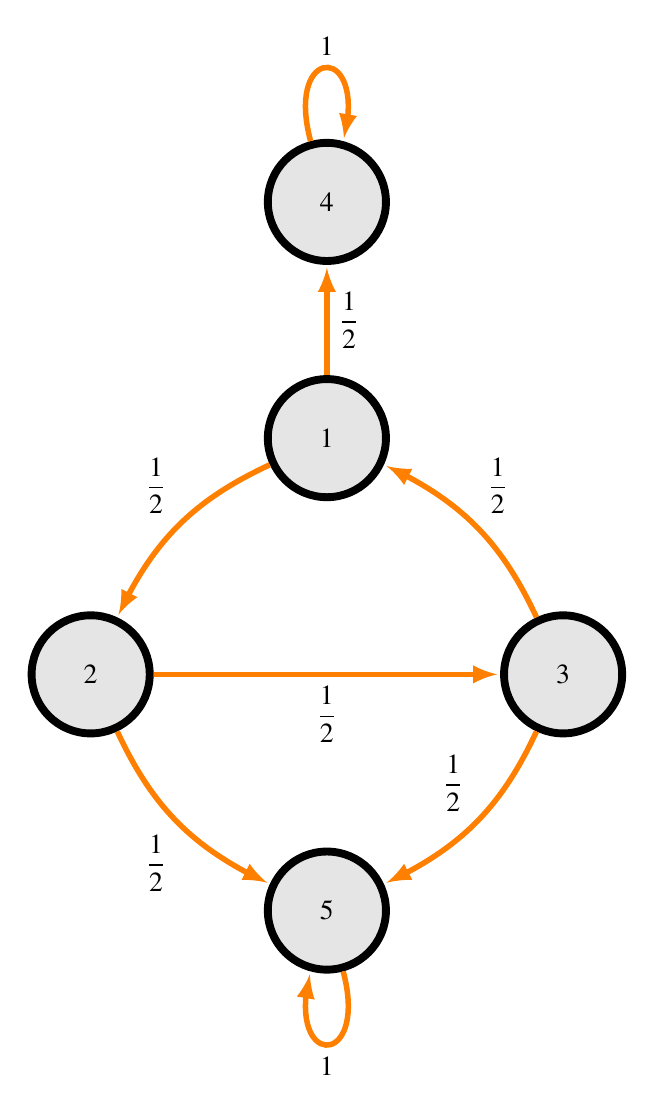
\begin{tikzpicture}
    % Setup the style for the states
        \tikzset{node style/.style={state, 
                                    minimum width=1.5cm,
                                    line width=1mm,
                                    fill=gray!20!white}}

        % Draw the states
        \node[node style] at (3, -3)      (bull)     {1};
        \node[node style] at (0, -6)      (bear)     {2};
        \node[node style] at (6, -6) (stagnant) {3};
        \node[node style] at (3, 0) (over1) {4};
        \node[node style] at (3, -9) (over2) {5};
        % Connect the states with arrows
        \draw[every loop,
              auto=right,
              line width=0.7mm,
              >=latex,
              draw=orange,
              fill=orange]
            (stagnant)     edge[bend right=20]            node {$\dfrac{1}{2}$} (bull)
            (stagnant)     edge[bend left=20]            node {$\dfrac{1}{2}$} (over2)
            (bull)     edge[bend right=20] node {$\dfrac{1}{2}$} (bear)
            (bull)     edge node {$\dfrac{1}{2}$} (over1)
            (bear)     edge[bend right=20] node {$\dfrac{1}{2}$} (over2)
            (bear)     edge node {$\dfrac{1}{2}$} (stagnant)
            (over1) edge[loop above]             node  {1} (over1)
            (over2) edge[loop below]             node  {1} (over2);
\end{tikzpicture}
\end{figure}

Theoretical vs Simulation plot
\centering
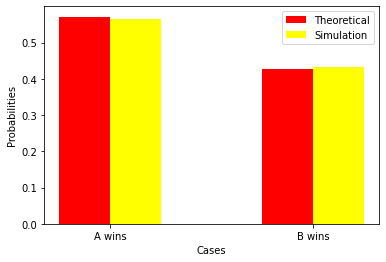
\includegraphics[scale=0.6]{Assignment8.png}








\begin{comment}


Then, the probability that someone wins at the $k^{th}$ trial is
\begin{align}
\tag{104.2}
\label{eq:exprsn}
    p_{X}(k)=pq^{k-1}
\end{align}
Let $Y \in \{ 1,2\}$ denote the winning player. $Y=1$ denotes $A$ wins, while $Y=2$ denotes $B$ wins.\\
From \eqref{table:1}, \eqref{eq:exprsn},
\begin{align}
\tag{104.3}
    p_{Y}(1)&=\displaystyle\sum_{m=0}^{\infty}p_{X}(3m+1)\\
\tag{104.4}
\label{eq:1}
    &=\displaystyle\sum_{m=0}^{\infty}pq^{3m}=\dfrac{p}{1-q^{3}}
\end{align}
\begin{align}
\tag{104.5}
    p_{Y}(2)&=\displaystyle\sum_{m=0}^{\infty}(p_{X}(3m+2)+p_{X}(3m+3))\\ 
\tag{104.6}
    &=\displaystyle\sum_{m=0}^{\infty}(pq^{3m+1}+pq^{3m+2})\\
\tag{104.7}
\label{eq:2}
    &=\dfrac{pq(1+q)}{1-q^{3}}
\end{align}
So,
\begin{align}
\tag{104.8}
\label{eq:3}
    p_{Y}(1)+p_{Y}(2)=\dfrac{p(1+q+q^{2})}{1-q^{3}}=\dfrac{p}{1-q}
\end{align}
Substituting \eqref{eq:0} in \eqref{eq:3}, we get
\begin{align}
\tag{104.9}
     p_{Y}(1)+p_{Y}(2)=1\\
\tag{104.10}
    \Rightarrow p_{Y}(1)=1-p_{Y}(2)
\end{align}
Solving \eqref{eq:1},\eqref{eq:2} with \eqref{eq:0}, we get
\begin{align}
\tag{104.11}
    p_{Y}(1)=&0.5714, p_{Y}(2)=0.4285\\
\tag{104.12}
    &\Rightarrow p_{Y}(1)>p_{Y}(2)
\end{align}



\newpage
 \\\\$P=$
$\begin{array}{c c} &
\begin{array}{c c c c} X_{1}  & X_{2} & X_{3} & X_{4}\\
\end{array}
\\
\begin{array}{c c c}
X_{1} \\
X_{2}\\
X_{3}\\
X_{4}
\end{array}
&
\left[
\begin{array}{c c c c}
0 & 0.5 & 0 & 0.5 \\
0 & 0 & 0.5 & 0.5 \\
0.5 & 0 & 0 & 0.5 \\
0 & 0 & 0 & 1  
\end{array}
\right]
\end{array}$
\\\\\\


\end{comment}
\end{document}